\section{Hauptteil}

\subsection{Tabelle}

\begin{center}
\tablehead{ \textbf{Head1} & \textbf{Head2} & \textbf{Head3}
\\ }
\bottomcaption[Beschreibung]{Beschreibung. Quelle: Berger, Vorlesung, 2012, München }
\begin{supertabular}{c|c|c}
\hline
1 & 2 & 3 \\
4 & 5 & 6 \\
7 & 8 & 9 \\
1 & 2 & 3 \\
4 & 5 & 6 \\
7 & 8 & 9 \\
\end{supertabular}
\end{center}

\subsection{Bilder}

\begin{figure}[H]
\begin{center}
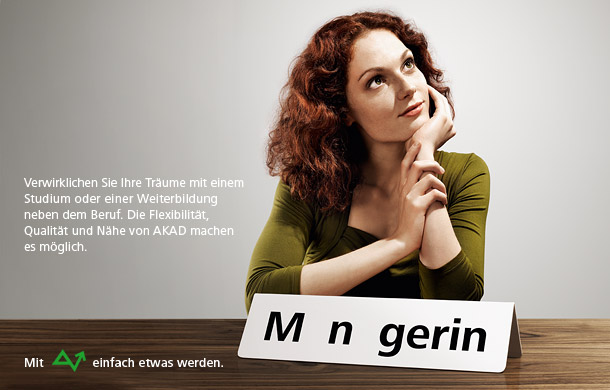
\includegraphics[scale=0.5]{akad_bild1.jpg}
\caption[Akad]{Akad. Quelle: www.akad.de}
\end{center}
\end{figure}

\subsection{Syntax Highlighting}
\begin{figure}[h]
\begin{minted}[bgcolor=bg]{php}
<?php 
$title="Lorem";
$desc = "Lorem Ipsum";
include($_SERVER['DOCUMENT_ROOT'].'/header.php'); 
?>
\end{minted}
\caption{Quellcode: Aufruf von header.php (PHP)}
\label{abb:header}
\end{figure}

